\section{Software beskrivelse}

For at danne overblik over software-udviklingen inden det egentlige design, anvendes N+1 modellen\footnote{4+1 architectural view model \url{https://en.wikipedia.org/wiki/4\%2B1_architectural_view_model}}. Denne beskriver fire faser som tager hånd om de overordnede ting inden for software, alt sammen med usecases som den røde tråd. De fire faser er:
\begin{enumerate}
    \item Logical View
    \item Deployment View
    \item Implementation View 
    \item Data View
\end{enumerate}
Disse punkter er beskrevet i detaljer herefter.

% Logical View
\subsection{Logical View}
Logical View skal danne et overblik over hvilke softwarepakker der befinder sig på platforme. Blokkene inde i de respektive pakker kan sammen med domænemodellen, hjælpe med at give et overblik over hvilke klasser og kernemoduler der skal bruges.
% Logical View Devkit8000
\subsubsection{Logical View Devkit8000}
\begin{figure}[H] \centering
    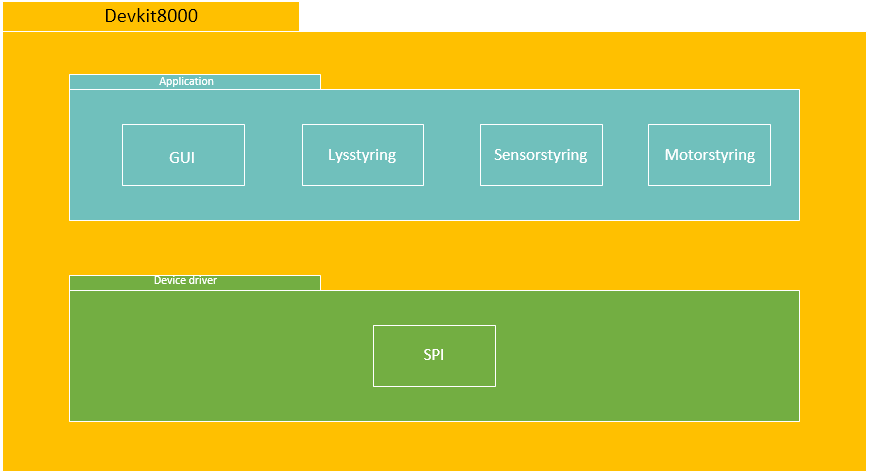
\includegraphics[width=\textwidth]{0_Filer/Figuer/LogicalViewDevkit8000.png}
    \caption{Logical View Devkit8000}
    \label{fig:LogicalView}
\end{figure}
Figur \ref{fig:LogicalView} illustrerer hvilke softwarepakker der ligger på Devkit8000. I bunden er Hardware API-pakken som håndterer protokol-vedtægter ifm. kommunikationen. I midten ligger Device drivers-pakken som håndterer protokol kommunikationen mellem Devkit8000 og PSoC. Application-pakken tager sig af alt UI samt kalibrering, sensorstyring og motorstyring.

% Logical View PSoC
\subsubsection{Logical View PSoC}
\begin{figure}[H] \centering
    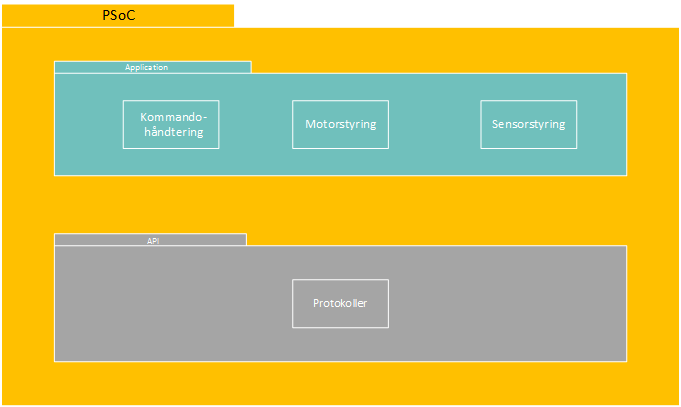
\includegraphics[width=\textwidth]{0_Filer/Figuer/LogicalViewPSoC.png}
    \caption{Logical View PSoC}
    \label{fig:LogicalViewPSoC}
\end{figure}
Figur \ref{fig:LogicalViewPSoC} illustrerer hvilke softwarepakker der ligger på PSoC. I bunden er en API-pakke som håndterer protokol-vedtægter ifm. kommunikationen. Øverst er application-pakken der tager sig af alt kommandohåndtering, motorstyring og sensorstyring.

% Deployment View
\subsection{Deployment View}
% DeploymentView
\subsubsection{DeploymentView}
\begin{figure}[H] \centering
    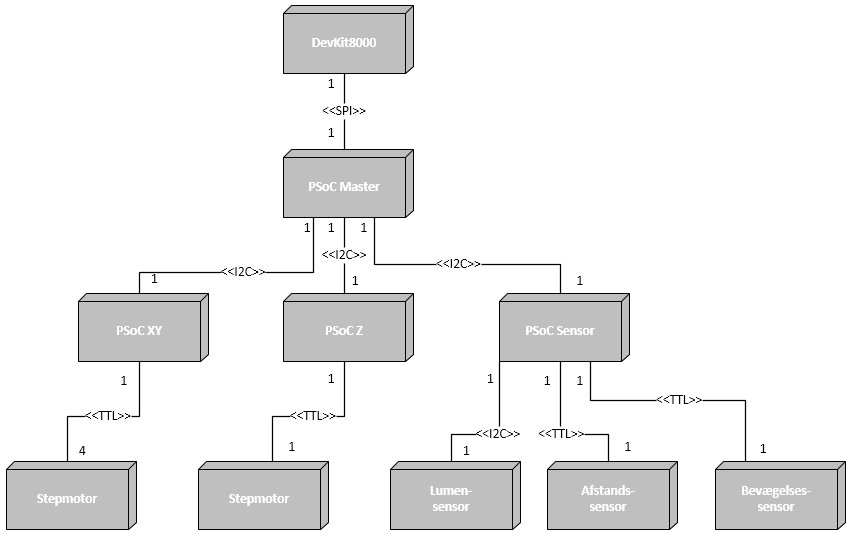
\includegraphics[width=\textwidth]{0_Filer/Figuer/DeploymentView.png}
    \caption{DeploymentView}
    \label{fig:DeploymentView}
\end{figure}


% Implementation View
\subsection{Implementation View}
Inden programmerne designes, fastlægges en struktur for kildekoden. På den måde er det nemmere for flere programmører at arbejde med delene i programmet samtidigt.
Strukturen skal være som vist i figur \ref{fig:ImplementationView}. Under mappen ”Kildekode” skal hver klasse have en mappe med dertil hørende filer. Ligeledes med ”Testprogrammer” mappen, som indholder testprogrammer som verificerer funktionaliteten af de enkelte moduler. Mappen ”Kompilerede programmer” er til de endelige programmer.
% Implementation View
\begin{figure}[H] \centering
    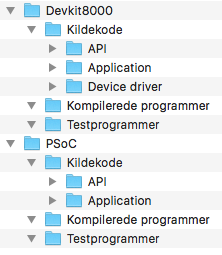
\includegraphics[width=0.4\textwidth]{0_Filer/Figuer/ImplementationView.png}
    \caption{Implementation View}
    \label{fig:ImplementationView}
\end{figure}


% Data View
\subsection{Data View}
I forbindelse med L.A.M.P. drift skal der gemmes data på en nem og håndterbar måde. Det skal være muligt at gemme følgende data:
\begin{enumerate}
    \item Position på X-motor
    \item Position på Y-motor
    \item Position på Z-motor
    \item Lysstyrke
    \item Lysets farve
    \item Kalibrerings data
\end{enumerate}